\documentclass[a4paper, 12pt]{article}
\usepackage{pgfplots}
\usepackage{xeCJK}
\begin{document}
直线边界，发射点在边界上，边界上粒子范围：$[0,2R]$；\\
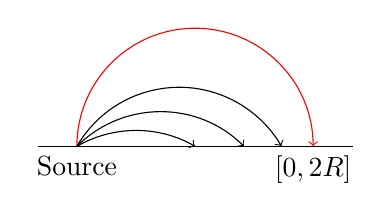
\begin{tikzpicture}
\coordinate (v2) at (0,0);
\coordinate (v1) at (4,0);
\draw  (v1) edge (v2);
\draw[->, red] (0.5,0) arc (180:0:1.5) node [below, pos=0, black] {Source} node [below, pos=1, black] {$[0,2R]$};
\draw[->] (0.5,0) arc (150:30:1.5);
\draw[->] (0.5,0) arc (120:60:1.5);
\draw[->] (0.5,0) arc (135:45:1.5);
\end{tikzpicture}\\
直线型边界，发射点在磁场内部，边界上粒子范围：$\sqrt{4R^2-d^2}$（直径做弦长）到$\sqrt{R^2-(R-d)^2}$（圆弧与边界相切）\\
\begin{tikzpicture}
\coordinate (v2) at (0,0);
\coordinate (v1) at (6,0);
\draw  (v1) edge (v2);
\draw[->, red] (3,1) arc (160:-20:1.5) node [below, pos=1, black] {$\sqrt{4R^2-d^2}$};
\draw[->] (3,1) arc (120:10:1.5);
\draw[->] (3,1) arc (20:-20:1.5);
\draw[->, red] (3,1) arc (-20:-90:1.5) node [below, pos=1, black] {$\sqrt{R^2-(R-d)^2}$};
\draw[->] (3,1) arc (-30:-120:1.5);
\draw[blue] (3,1) -- (3+2*1.414,0);
\draw[blue] (3,1) -- (3-1.414,1);
\draw[blue] (3-1.414,1.5)--(3-1.414,0);
\draw[blue] (3-1.414,1.5)--(3,1);
\draw[red] (3,1) -- (3,0) node [right, pos=1] {最短时间};
\fill (3+1.414, 0.5) circle (1pt);
\fill (3-1.414, 1.5) circle (1pt);
\end{tikzpicture}\\
条形边界，并且宽度$d\in (r,2r)$。此时两条边界都有粒子射出，上边界范围长度：$2\sqrt{R^2-(d-R)^2}$，左侧通过勾股定理与射出方向向左进行求解，右侧通过相切求解，左右长度相同。\\
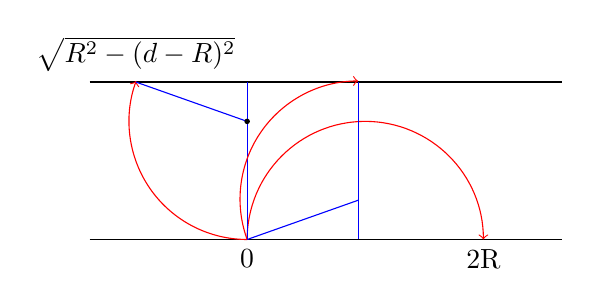
\begin{tikzpicture}
\coordinate (orig) at (0,0) node [below]{0};
\draw (-2,0) -- (4,0);
\draw (-2,2) -- (4,2);
\draw[red, ->] (0,0) arc (180:0:1.5) node [pos=1, below, black] {2R};
\draw[red, ->] (0,0) arc (-90:-200:1.5) node [pos=1, above, black] {$\sqrt{R^2-(d-R)^2}$};
\draw[blue] (0,0) -- (0,2);
\draw[blue] (0,1.5) -- (-1.414, 2);
\fill (0,1.5) circle (1pt);
\draw[red, ->] (0,0) arc (200:90:1.5);
\draw[blue] (1.414,0) -- (1.414,2);
\draw[blue] (0,0) -- (1.414, 0.5);
\end{tikzpicture}\\

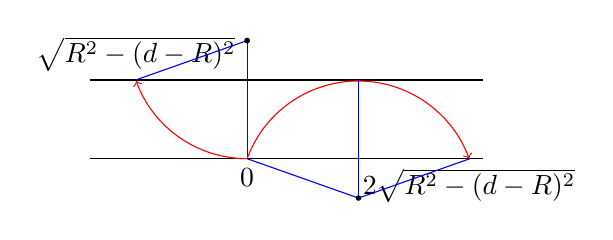
\begin{tikzpicture}
\coordinate (orig) at (0,0) node [below]{0};
\draw (-2,0) -- (3,0);
\draw (-2,1) -- (3,1);
\draw[red, ->] (0,0) arc (-90:-160:1.5) node [pos=1, above, black] {$\sqrt{R^2-(d-R)^2}$};
\draw[blue] (0,0) -- (0,1.5);
\draw[blue] (0,1.5) -- (-1.414, 1);
\fill (0,1.5) circle (1pt);
\draw[red, ->] (0,0) arc (160:20:1.5) node [pos=1, below, black] {$2\sqrt{R^2-(d-R)^2}$};
\draw[blue] (1.414,-0.5) -- (1.414,1);
\draw[blue] (0,0) -- (1.414, -0.5);
\draw[blue] (2*1.414,0) -- (1.414,-0.5);
\fill (0,1.5) circle (1pt);
\fill (1.414, -0.5) circle (1pt);
\end{tikzpicture}\\

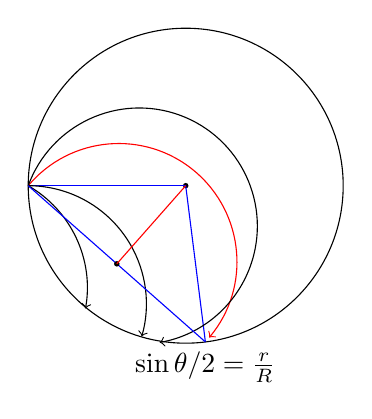
\begin{tikzpicture}
\coordinate (orig) at (0,0){};
\fill (0,0) circle (1pt);
\draw [blue] (0,0) -- (-2,0);
\draw [blue] (0,0) -- (0.25, -1.984);
\draw (0,0) circle (2);
\draw[->, red] (-2,0) arc (140:-40:1.5);
\draw[->] (-2,0) arc (160:-80:1.5);
\draw[->] (-2,0) arc (90:-16:1.5);
\draw[->] (-2,0) arc (60:-10:1.5);
\draw[blue] (-2,0) -- (0.25, -1.984) node [pos=1, black, below] {$\sin\theta/2=\frac rR$};
\fill (-0.875, -0.992) circle (1pt);
\draw [red] (0,0) -- (-0.875, -0.992);
\end{tikzpicture}\\

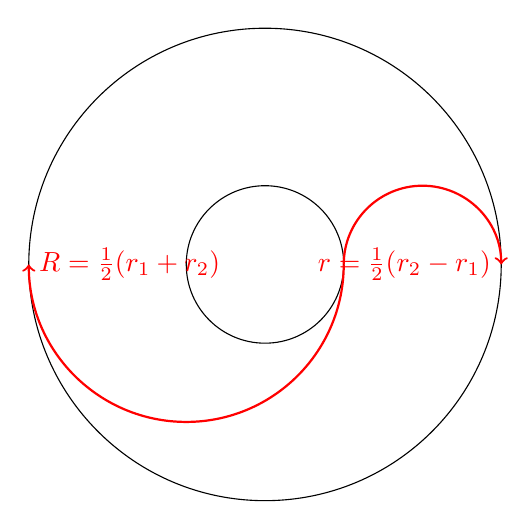
\begin{tikzpicture}
\coordinate (orig) at (0,0){};
\draw (0,0) circle (3);
\draw (0,0) circle (1);
\draw [red, ->, thick] (1,0) arc (180:0:1) node [pos=1,below, left] {$r=\frac12(r_2-r_1)$};
\draw [red, ->, thick] (1,0) arc (0:-180:2) node [pos=1,above, right] {$R=\frac12(r_1+r_2)$};
\end{tikzpicture}
\end{document}